% --------------------------------------------
%		CHAPTER 1
%---------------------------------------------

\chapter{Belle II and SuperKEKB (SKB) accelerator}
%\addcontentsline{toc}{chapter}{Belle II e acceleratore SKB (SuperKeKB)}

\begin{comment}
In this first chapter we will see a summary of the principal physics measurements conducted (?? taken) by Belle II experiment, focusing on the ones which could take particularly advantage from the upgrade of the vertex detector, discussed in this work. We will also go through the structure and the operation of the SuperKEKB accelerator and Belle II detector, to conclude (end) with a short view on the actual state of measurements.
\end{comment}

In this first chapter we will see a summary of the principal physics measurements on which the Belle II collaboration concentrates its efforts, focusing on the ones which could take particularly advantage from the upgrade of the vertex detector, discussed in this work. We will also go through the structure and the operation of the SuperKEKB accelerator and Belle II detector, to conclude with a short view on the actual state of measurements.




%---------------------------------------------
%			1.1
%---------------------------------------------
\section{Physics program of the B-factories}
%\addcontentsline{toc}{section}{Programma di fisica alle B-Factory}


%REFERENCE BIBLIO [PHYSICS BOOK]

Belle II is a general-purpose spectrometer, committed to making precision measurements of the Standard Model's parameters (SM) and to looking for the physics Beyond the Standard Model (BSM).
In particular the experiment studies the Charge-Parity Violation (CPV) in the B mesons system and it also searches for New Physics (NP) evidences in the decays of B and D mesons, in $\tau$ leptons and in the dark matter sector (DM), above all hunting for dark photons.

\subsection{Opened questions in SM}

The SM is a physics theory that describe three of the fundamental interactions involving elementary particles, which are strong, weak and electromagnetic interaction (with the exclusion of the gravitational one). It classifies all known particles up to now in 4 main groups: quark, leptons, bosons and Higgs (figure ~\vref{fig:sm}).


\begin{figure}[h]
\centering
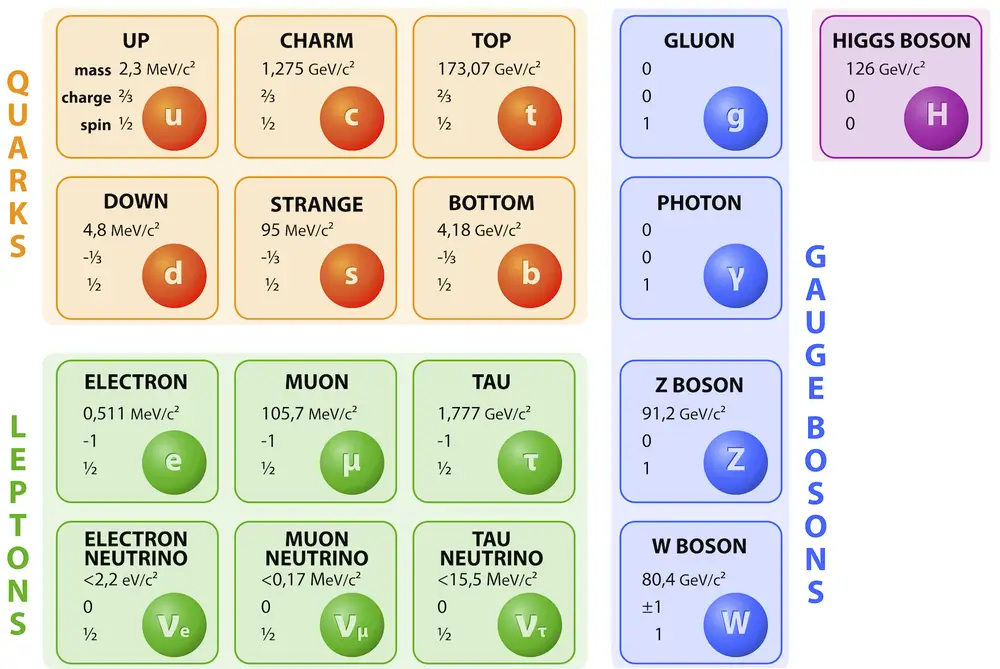
\includegraphics[scale=0.3]{SM}
\caption{Particle classification in the Standard Model}
\label{fig:sm}
\end{figure}

Despite its tremendous success achieved over the years, predicting with high precision new particles and mechanisms unknown until that moment, there are many aspects of the Nature, on which it is unable to give answers. Some of them are listed in the following.

\begin{itemize}
\item Three generations of quark and leptons are known, but it is not known wheter they should be the only ones and the reasons behind their mass hierarchy.
\item Higgs mechanism is able to explain the cause of elementary particles' masses through spontaneous electro-weak symmetry breaking, but it doesn't justify those of neutrinos.
\item The SM also predicts other Higgs-like bosons, potentially vector bosons, whose existance would be justified in some SUper-SYmmetry (SUSY) theories or others of New Physics.
\item Another opened question is the matter-antimatter asymmetry in the Universe. Even though CP violation is necessary to explain the current state of the universe, the observed quantity is several orders of magnitude less than needed to explain the matter domination over antimatter, which have allowed the evolution of the universe as we know it today.
\item The elements of the Cabibbo-Kobayashi-Maskawa (CKM) matrix, which complex phase is at the foundation of CP Violation (CPV) in the quark flavor sector, are diagonal e it could be suggested the existance of a new symmetry, that exists unbroken at high energy (greater than the order of TeV).
\end{itemize}

All these opened questions encourage the research of new particles and processes that could give reasonable answers.\\
At the energy frontier, experiments like the Large Hadron Collider (LHC) in Geneve are looking for new particles created from the proton-proton collision with a center mass energy up to 14 TeV.\\
At luminosity frontier instead, the trace of new particles and mechanisms is searched in precision measurements of suppressed reactions in flavour physics or in the deviations from SM. The discrepancies indeed, could be interpreted as a clue of new physics beyond SM. The last is the Belle II approach.\\
Moreove new physics models searched in Belle II are those that include more specific flavor couplings, from which indirect seraches can push the new physics scale much higher than the direct search programs.


% \subsection{Ricerche di nuova fisica (BSM)}
\subsection{Belle II Physics channels}

In the following we will see the main physics channels of Belle II, focusing on those that would benefit the most from the upgrade of the whole detector and in particular of the vertex detector.\\

\hspace{.2cm}

\textbf{FLAVOR PHYSICS}
\begin{description}
\item [CP-violating phases in quark sector:]\
	\begin{itemize}
	%\itemsep0em
	\item as we mentioned above, the amount of CP violation in the SM is not enough to explain the difference observed between baryon-antibaryon matter. New clues of CPV could be found studying the discrepancy between $B^{0}$ and $\bar{B_{0}}$ decay rates, so measuring the time-dependent CP violation in penguin transition of  b $\rightarrow$ s and  b $\rightarrow$ d quarks (such as B $\rightarrow$ $\phi K^{0}$ and B $\rightarrow$ $\eta' K^{0}$). In fact this violation is expected to be very small in the SM, so any significant observation of CPV can be interpreted as a signal beyond the SM.
	\item Also the CP violation in charm mixing, negligible in the SM, could draw attention to new phenomena in the up-type quark sector.
	\item Another aspect that need to be understood is the large amount of CP violation in the time-integrated rates of charmless hadronic B decays, such as B $\rightarrow$ $K\pi$ and B $\rightarrow$ $K\pi \pi$, observed by other B factories and LHCb. 
	\end{itemize}

Conclusive measurements of time-dependent CP violation require a combination of data size and high precision measurement of $\Delta z$ (reference in paragraph), the distance between the tag and signal in B meson decay vertices. In this respect, the upgrade of the vertex detector could improve a lot the flavor tagging efficiency losses, due to the beam-induced backgrounds, among the others.

\item[Multiple Higgs bosons:] Another fundamental channel is the measurement of the Branching Ratio (BR) of B $\rightarrow$ $\tau\nu$, which is particularly sensitive to the charged Higgs boson (in addition to a neutral SM-like Higgs) that in general couples more strongly to heavier particles. But also the BR of the decay B $\rightarrow$ $D^{(*)}$$\tau\nu$, where BaBar, Belle and LHCb had already reported some anomalies. Moreover extended Higgs mechanism could introduce extra sources of CP violation.
We could notice that semi-tauonic decay measurements, rely on efficient and pure tag side B full reconstruction, and so also on the performance of the Vertex Detector.
\begin{comment}
In general the detection of b $\rightarrow$ $\tau$ $\rightarrow$ \textit{l} transitions requires good lepton identification below 700 MeV/c (Low momentum track finding).
\end{comment}

\item[Flavor Changing Neutral Current (FCNC):]\
	\begin{itemize}
	%\itemsep0em
	\item For this purpose, measurements of time-dependent CP violation in (...), triple product CP violation asmmetrie in B $\rightarrow$ VV decays, and semileptonic decays B $\rightarrow$ V\textit{l}$\nu$, V= $D^{*}$, $\rho$ are the main approaches. 
	\item It is also important measure b $\rightarrow$ s$\nu\bar{\nu}$ transitions (such as...) which belong to a class of decays with large missing energy. 
	\item???? Moreover it's necessary to improve FCNC measurements of b $\rightarrow$ d, b $\rightarrow$ s, and c $\rightarrow$ u transitions. 
	\end{itemize}
	
Most analyses with missing energy in the final state utilise hadronic or semileptonic B full reconstruction techniques and the performance of these method is most dependent on low momentum track finding and so on the capabilities of the vertex detector as well.

\item [Sources of Lepton Flavor Violation (LFV):] LFV in charged lepton decay (at rates of $10^{-8}$) is a key prediction in many neutrinos mass generation mechanism and other models of physics BSM. Belle II has an unrivalled sensitivity to $\tau$ decays, because of their production in a clean $e^{+}e^{-}$ collision background and the large dataset. The experiment analyze $\tau$ leptons to search for LF and CP violation and measurement of the electric dipole moment and (g-2) of the $\tau$.

\end{description}

\hspace{.2cm}

\textbf{NON FLAVOR PHISICS}

\begin{description}
\item[Dark Sector:] Belle II has a unique sensitivity to dark matter via missing energy decays. Although most research for NP are indirect, there are different model that predict the existance of new particles at the MeV to GeV scale, that couple to the SM via new gauge asymmetries. They also predict a vast range of hidden particles, including dark matter candidates and new gauge bosons.

In these last two areas, $\tau$ and dark sectors physics, the aim is to probe forbidden and ultra-rare transition in low-multiplicity final states with as large dataset as possible. This is mostbly rely on trigger efficiency and new trigger strategies, that could take advantage from the upgrade. Many of these processes can only be accesed at Belle II, so it is fundamental increase the perfomance of the detector.

\item[Binding Hadrons:] As time goes on, in other B factories and hadron colliders, a large numbers of states not predicted by conventional mesons interpretation are discovered, changing our understanding of QCD in the low-energy regime. For this reason, study of quarkonia is a fundamental purpose for Belle II. In fact new particles can be produce near resonance, achievable by adjusting the machine energy, or by intial state radiation, which effectively provides a continuum of center of mass energies. 

\item[CKM matrix:] Belle II is also dealing with the measurements of CKM observable, the matrix elements and their phases, with unprecedented precision. 

\end{description}


\subsection{B meson decay vertices}

IMPORTANZA DEI VERTICI SECONDARI


%METTI REFERENCE PHYSICS BOOK AND UPGRADE ARTICLE
\newpage





%---------------------------------------------
%			1.2
%---------------------------------------------
\section{SuperKEKB accelerator}
%\addcontentsline{toc}{section}{Acceleratore SuperKEKB}

%%%%%%%%%%%VEDI ARTICOLO SU BKG

The Belle II sensitivity in the precision measurements that we sift throug in the previous section, is feasible expecially thanks to the extraordinary performance of the SuperKEKB accelerator which host the (almost) hermetic detector. This complex facility is the result of efforts and efficient collaboration between the researches of KEK laboratory and all the international working groups that partecipate(take part, contribute) to the experiment.

%\subsection{SuperKEKB and luminosity}
\subsection{The facility}

SuperKEKB is an asymmetric $e^{+}e^{-}$ collider with a circumference of 3 km, and a center of mass energy peak equal to  $\sqrt{s}$ = 10.58 GeV, which corresponds to the mass of the $\Upsilon(4S)$ resonance.
Compared to its predecessor KEKB (which started its operation in 1998 and concluded in 2010), the current accelerator has allowed to obtain the highest luminosity ever achieved, equal to \num{4.7e-34} $cm^{-2}s^{-1}$ in July 2022, using a new scheme to accelerate and collide the beams, the so called \textit{nano-beam scheme}(reference). [This was made possible through some improvements and additions in the components of the accelerator itself]. Moreover the new upgrade of the machine, still under study, will also include (provide for) other intervention expecially to cope with higher background level, in view of further increase of the luminosity.

\begin{figure}[h!]
\centering
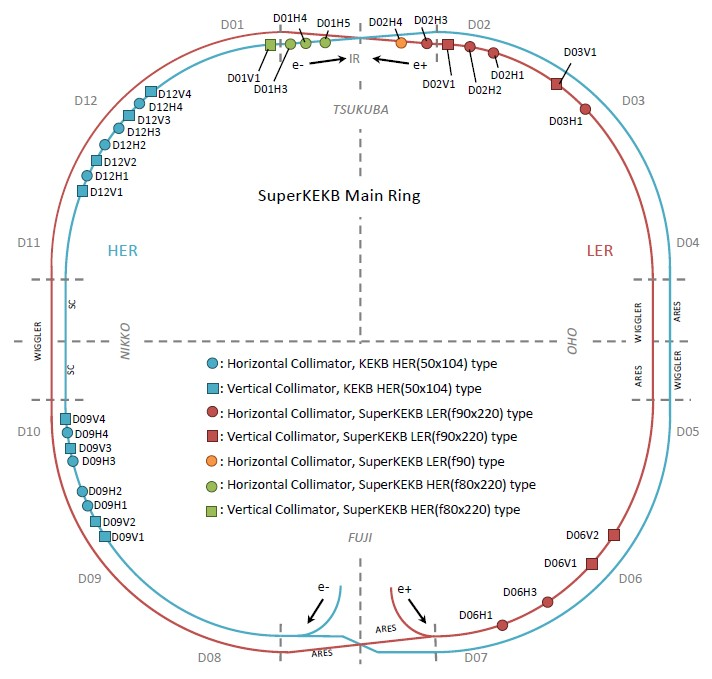
\includegraphics[scale=0.7]{SuperKEKB}
\caption{SuperKEKB accelerator in 2021. The letters V and H denote respectively vertical and horizontal collimators. Each ring is divided in 12 sections, from the first called D01 to the last D12.}
\label{fig:superkekb}
\end{figure}


We will briefly see the main features and parameters of the accelerator.\\
%%struttura meccanica(lunghezza, fasci, etc...)

\textbf{Luminosity}\\

Luminosity is one of the key parameters of an accelerator, it represents the interaction rate per unit of cross section between colliding particles:

\begin{equation}
L =\frac{1}{\sigma}\frac{dN}{dt} 
\end{equation}

from which, reversing the equation to obtain N, namely the number of observable physical events:

\begin{equation}
N = \int_{0}^{T} L\sigma dt
\end{equation}

where T is the duration of the experiment,  $\sigma$ the cross section of the physical process of interest.
(Specifically) In particular luminosity is strictly dependent from machine parameters and from the main characteristics of the beam. With respect to this, it can be expressed as:

\begin{equation}
L = ..................
\end{equation}

where ......

\hspace{.1cm}
As we have already seen, SuperKEKB holds the actual world record in luminosity, with a peak of \num{4.7e-34} $cm^{-2}s^{-1}$ with $\beta^{*}_{y}$= 1.0 mm. In the near future the target will be to reach a luminosity of \num{6.3e-35} $cm^{-2} s^{-1}$, increasing current beams and reducing their section in the Interaction Point (IP), squeezing the betatron function up to a value of $\beta^{*}_{y}= 0.3$ mm.\\
For these reasons, the supervision of the beams background becomes one of the most important aspect both to reach the goal and to improve the possible precision measurements of physics. 

At present (currently) it is estimated that the background should remain accettable up to a luminosity value equal to \num{2.8e-35} $cm^{-2} s^{-1}$ with $\beta^{*}_{y}$= 0.6 mm.
As we shall see, the possibility(hope) to achieve higher luminosity is closely (strictly) relate to an upgrade plan of both the detector and the accelerator.

\hspace{.2cm}


\textbf{Beam energy}\\

%METTI REFERENZA '' Beam bkg expectation (A)''

Energy beams is mostly decided by the physics program interesting for the experiment. Currently SuperKEKB collides an electron beam with energy of 7 GeV (High Energy Ring, HER) , with a positron beam of 4 GeV (Low Energy Ring, LER), reaching a center of mass energy peaked to $\Upsilon$(4S) resonance.\\
Also the choice of colliding (using) asymmetric beam (like its predecessor KEKB, which collided (got collide) electrons beam of 8 GeV with a positrons beam of 3.5 GeV) is necessary to identify and measure decay vertices of particles created in the collision (paragraph reference). We have already seen some of the physics behind this choice in section..... [We can notice that the different balance between beam energies (lower beam energy in HER, higher in LER respect to KEKB) was chosen to reduce the beam losses due to Touschek scattering in the LER. This is expected to reduce the spatial separation between B mesons, studied in time-dependent CPV measurements, but leads to slight improvements in solid angle acceptance for missing energy decays].\\
Indeed this mechanism allows to boost the decay products, improving the vertices reconstruction and increasing the sensitivity of the physics measurement, too. In particular this makes possbile time-dependet measurements, expecially in CP violation.

%%VEDI COME E' NECESSARIO NELLE MISURE DI FISICA

In figure \vref{beame} the flexibility of the energy of both beams LER and HER is showed. The possible range covers energies which goes from the $\Upsilon$(1S) (9.46 GeV) resonance to the $\Upsilon$(6S) (11.24 GeV), with a peak in 11.24 GeV.

\begin{figure}
\centering
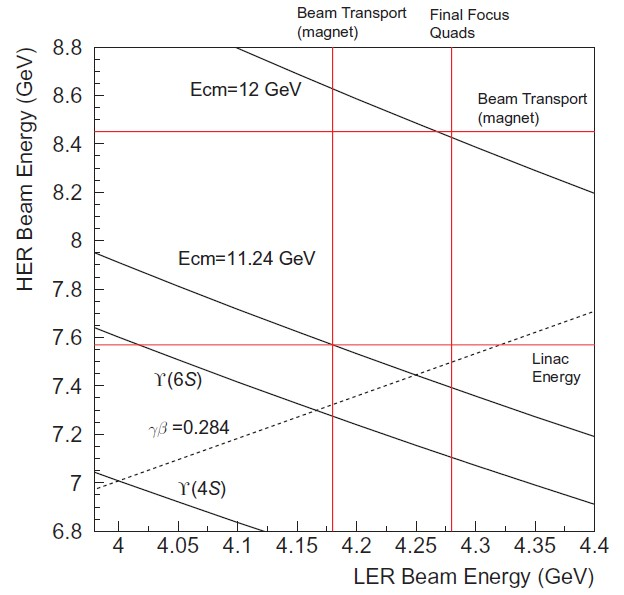
\includegraphics{beam_energy}
\caption{Beam energies to reach center of mass energy equal to $\Upsilon$(4S), $\Upsilon$(6S), 11.24 GeV and 12 GeV. Horizontal axis represents the energy of LER and the vertical one the energy of HER. }
\label{fig:beame}
\end{figure}

%%%%%aggiungi cosa permette


\subsection{''Nano-beam'' scheme} [?]

As mentioned in the previous section, a key element to define the luminosity is the \textit{beta function} $\beta$ in the Interaction Point (IP). To be able to increase luminosity, it's necessary to decrease the value of $\beta$ depending on the variation of the other machine parameters, but not only, which are part of its definition (richiama equazione con parametri macchina).
The mechanism used in SuperKEKB is called \textit{nano-beam scheme}, and it allowed to obtain luminosity 40 times greater than that of KEKB, managing to (succeding) decrease of 1/20 the $\beta$ function in the IP.

This new scheme, designed by P. Raimondi, dictates that the beams collide at large angle, in SuperKEKB equal to 83 mrad (keeping beams divided through quadruople magnets), in order to reduce the \textit{hourglass effect}, which succeed when the bunches in the beam are much longer.\\
We can see briefly the most important parameters that influnce the mechanism?????

The overlap area of the beams is localized and its lenght is given by:

\begin{equation}
d = \frac{\sigma_{x}^{*}}{sin\phi_{x}}
\end{equation}

with $\phi_{x}$ defined as half of the crossing angle. The overlap lenght d represent the real lenght of the bunch to consider in the evaluation of the hourglass effect, and it is smaller than the effective bunch lenght along the direction of the beam axis. To reduce this effect, it's necessary to get:

\begin{equation}
\beta_{y}^{*} \geq d = \frac{\sigma_{x}^{*}}{sin\phi_{x}}
\end{equation}

Therefore to increase the $\beta$ function in the IP, the value of d has to diminish, decreasing as aconsequence the horizontal section in the IP and also icreasing the crossing angle.
Using a crossing angle large enough, has other positive implications on the operation of the accelerator:

\begin{itemize}
\item allows the placement of a new focusing system in the IP with a superconducting quadrupole magnet;
\item allows to have two distinct line which host HER and LER beams;
\item diminisches the \textit{fringe fields} effect in the IP, wihch are the residuals of the magnets (magnetic fields) in the proximity (nearby). 
\end{itemize}

In figure \vref{fig:beampar} are reported the main machine parameters (default value) of the SUperKEKB accelerator.

\begin{figure}
\centering
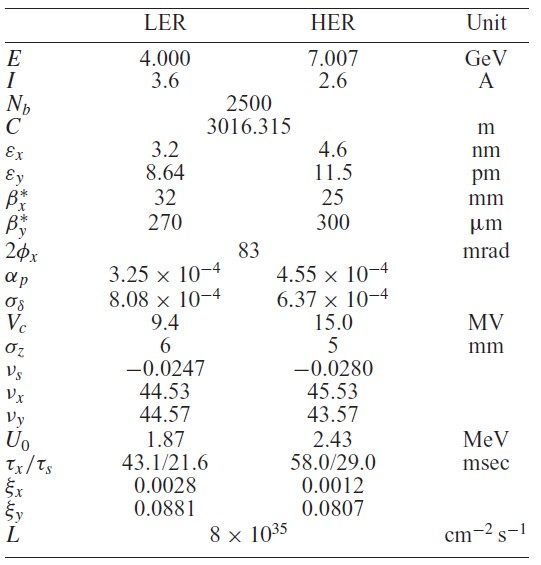
\includegraphics{beam_par}
\caption{Machine parameters of SuperKEKB. The mark ''*'' indicate values in the IP.}
\label{fig:beampar}
\end{figure}

%%%%%% CRAB WAIS COLLISION SCHEME

%PARLARE DELLA COSA ORIZZONTALE???

\newpage



%---------------------------------------------
%			1.3
%---------------------------------------------
\section{Belle II detector}
%\addcontentsline{toc}{section}{Il rivelatore Belle II}

Belle II detector is a general-purpose spectrometers, optimized in precision measurements of B mesons and their decay products. Compared to its predecessor Belle, it have to preserve (mantain) good performance despite having smaller boost in the center of mass and suffering greater levels of backgrounds and so of radiations, which are one of the main causes of premature degradation of performance and expected mean life of the detector itself.\\

Belle II consists of a series of nested subdetectors, which surrounds the IP of the two beams, placed around the berillium beam pipe of 1 cm(10 mm??) of radius. Now we will go trough a briefly description of the several subdetectors. 

% METTI IMMAGINE

\subsection{Vertex Detector (VXD)}

The \textbf{VerteX Detector (VXD)} is composed by two devices, the silicon Pixel Detector (PXD) and the Silicon Vertex Detector (SVD), for a total of six layers around the beam pipe.
PXD('s) two first layers (at a radius of 14 mm and 22 mm, respectively) consist of pixelated sensors of the DEPFET type. The remaining four layers of SVD instead, are equipped with double-sided silicon strip sensors (at 39 mm, 80 mm, 104 mm and 135 mm respectively). 

\subsection{Central Drift Chamber (CDC)}

It is the central tracking device, with a large-volume drift chamber and small drift cells. The chamber gas is comprised of a \ch{He-C_{2}H_{6}} 50:50 mixture with an average drift velocity of 3.3 $\mu s^{-1}$ and a miximum drift time of about 350 ns for a 17 mm cell size.
The CDC contains 14336 wires rranged in 56 layers either in \textit{axial} orientation (so aligned with the solenoidal magnetic field) or \textit{stereo} (skewed with respect to the axial wires). In fact by combining information from both the axial and the stereo layers it is possible to reconstruct a full three-dimensional helix track.

%immagine

% In order to operate at high events rates with increased backgorund levels in fact, 

\subsection{Particle identification system (TOP e ARICH)}

\textbf{TOP} is a special kind of Cherenkov detector where the two-dimensional information of a Cherenkov ring image is given by the time of arrival and impact position of Cherenkov photons at the photodetector at one end of a 2.6 m quartz bar. It is composed by 16 detector module and each one (of them) consists of a 45 cm wide and 2 cm thick quartz bar with a small expansion volume (about 10 cm long) at the sensor of the bar. At the exit window of the wedge, two rows of sixteen fast multi-anode photon detectors are mounted. This detector requires microchannel plate (MCP) photomultiplier tubes (PMT) specially dveloped for this purpose.\\

\textbf{ARICH} is used to identify charged particle and it is placed in the forward endcap region. It is a proximity focusing Cherenkov ring imagine detector with aerogel as Cherenkov radiator. The number of detected Cherenkov photons is a key parameter of the RICH and in this experiment it is increased by a novel method. Two 2 cm-thock layers of aerogel with different refractive indices (n = 1.045 upstream, n= 1.055 downstream) are used to increase the yield without degrading the Cherenkov angle resolution.
As the single-photon-sensitive high-granularoty sensor, a hybrid avalanche photon detector (HAPD) is used.  

\subsection{Electromagnetic calorimeter (ECL)}

The \textbf{ECL} is a highly segmented array of tallium-doped caesium iodide CsI(Tl) crystals assembled in a (projective geometry). THis detector is used to detect gamma rays and to identify electrons, and in particular to separate electrons from hadrons (expecially pions). All three detector regions (barrel, forward and backward endcaps) are instrumented with a total of 8736 crystal, covering about 90 \% of the solid angle in center-of-mass system.

\subsection{$K_{L}$ muon detector (KLM)}

It consists of an alternating sandwich of 4.7 cm-thick iron plates and active detector elements located outside the superconducting solenoid. The iron plates serve as the magnetic flux return joke for the solenoid. They also provide 3.9 interaction lenghts or more of material, beyond the 0.8 interaction lenghts of the calorimeter, in chich $K_{L}^{0}$ mesons can shower hadronically. The active detector elements have been chosen in order to cope with the reduction of the detector efficiency under the SuperKEKB background rates. Layers of scintillator strips with wavelenght-shifting fibers are used, the readout instead relies on silicon photomultipliers (SiPMs, Geiger mode operated APDs(...)) as light sensors.

\subsection{Trigger system}

The trigger system of Belle II has a non-trivial role to identify eventsof interest during data-taking. It must work efficiently in the presence of high background rates, while respecting (satisfying) the limitations of the DAQ (?).
This system is composed of two levels: a hardware-based low-level trigger (L1) and a software-based high-level trigger (HLT). 

\begin{itemize}
\item \textbf{L1}: has a latency of 5 $\mu$s and a maximum trigger output rate of 30 kHz, limited by the read-in rate of the DAQ.
\item \textbf{HLT}: is a key component of the DAQ and it has to reduce online event rates to 10 kHz for offline storage, and it must identify track regions of interest for PXD readout in order to reduce data flux. It reconstructs events with offline reconstruction algorithms, using all detectors infromation except for the PXD.
\end{itemize}

%VEDI ANCHE ARTICOLO GIULIANA
%TABELLA CON SUMMARY DA PHYSICS BOOK?




\newpage




%---------------------------------------------
%			1.4
%---------------------------------------------
\section{Current state and perspectives of data taking}
%\addcontentsline{toc}{section}{Stato attuale e prospettive delle prese dati}



%%%% 	Luminosità raggiunte e statistica?
%%Belle II online luminosity & record luminosità istantanea
%% doev si vuole arrivare 50 abinv e come??
%% cose achved nelle previsioni parametri di macchina dell'articolo B

%ARTICOLO B: there are two major upgrades of the machine plannd in the next ten years:....





%--------------------------------------------------
%		bibliography
%--------------------------------------------------
% 1. 	PHYSICS BOOK
%2. 	UPGRADE ARTICLE
%3. 	Background SuperKEKB article



%%%%%%%%%%%%%%%%%%%%%%%%%%%%%%%%%%%%%%%%%%%%%%

\begin{comment}

\subsection{Alcune ulteriori modifiche rispetto a KEKB}

L'upgrade da KEKB a SuperKEKB, come in parte visto, ha richiesto importanti cambiamenti nei fasci e nello schema di collisione, tutto volto a raggiungere nuove vette di luimnosità. Altre fondamentali modifiche sono state fatte lungo l'anello di collisione, tra cui:

\begin{item}
\item rifacimento della regione d'interazione, che comprende 4 m intorno al PI, in modo da poter ospitare il nuovo detector Belle II, il sistema di focusing finale dei fasci e le due beam pipes;
\item il sistema a radiofrequenza è stato modificato per permettere una corrente maggiore dei fasci;
\item l'aggiunta di alcuni collimatori lungo entrambi gli anelli (11 nel LER  e 20 nel HER) per poter limitare il danno da radiazione sul rivelatore e i ''quenches'' dei magneti superconduttori, cioè un surriscaldamento dei suoi avvolgimenti che genericamente causa la perdità della superconduttività, dissipando la corrente circolante.
\item anche il sistema di vuoto è stato migliorato per limitare alcuni effetti collegati alla perdita di potenza del fascio, allungando quindi la vita media del fascio stesso.
\end{item}

\end{comment}


%%%%%%%%%%%%%%%%%%%%%%%%%%%%%%%%%%%%%%%%%%%%%

\begin{comment}

\subsection{Background monitoring system} [?]
%% Per le sorgenti di rumore si rimanda al capitolo 2 o lo metti nel capitolo 2?

Background is one of the most important problem for a particle detector, both for precision measurements of physics and for the performance of the different layer detector which constitute (make up) Belle II. For this reason several detectors are used to obtain measurements of radiation dose on both detector and delicate regions of the accelerator, to intervene as soon as possible in case of too high levels are reached. Indeed large doses of radiation could cause accidental damages on the detector, decreasing its performance.

In the chapter 2 (reference) we will go through the main (primary, leading) reasons of background. For now we mention some of the monitoring devices for the backgorund in SuperKEKB.


\begin{itemize}
\item Diamonds detector (called ''Diamonds') which control the rate of the radiation dose in the interaction region of the beam pipe. These also are part (take part) of the ''fast beam abort system'', which is a control system that collect (consider) data from different detector to evalute (valutare nel senso di decidere) the beam ''turning off'', in order to avoid that events out of control could cause damage (harm) to the whole structure.
\item CLAWS (sCintillation Light And Waveform Sensors), made by scintillator of plastic material and silicon photomultipliers, and used to monitor the Belle II background in the nearby (proximity) of the beam injection (main ring). Together with diamonds it takes part to the beam-abort system.
\item TPC's (Time Projection Chambers) which provides measurements (better) on the direction of the neutron flux in the tunnel which hosts (that houses) the accelerator.
\item $He^{3}$ tubes for the counting of thermal neutrons (which are those with a kinetic energy lower than 1/10 of eV, generally about 0.025 eV) around the Belle II detector.
\end{itemize}

\end{comment}
